%-------------------------------------------------------------------------------
%   PACKAGES AND OTHER DOCUMENT CONFIGURATIONS
%-------------------------------------------------------------------------------


\documentclass[a4paper,12pt]{article}
\usepackage[english]{babel}
\usepackage[latin1]{inputenc}
\usepackage{amsmath}
\usepackage{amssymb}
\usepackage{amsfonts}
\usepackage{graphicx}
\usepackage{lipsum}
\usepackage[colorinlistoftodos]{todonotes}
\usepackage[toc,page]{appendix}
\usepackage{setspace}
\usepackage{tcolorbox}
\usepackage{bbm}
\tcbuselibrary{skins}
\doublespacing
\usepackage{booktabs}
\usepackage[parfill]{parskip}
\usepackage{hyperref}
\usepackage{geometry}
\usepackage[bottom]{footmisc}
\usepackage{longtable}
% \usepackage[demo]{graphicx}
\usepackage{subfig}
\usepackage{multirow}
\usepackage{tikz}
\usetikzlibrary{fit}
\usetikzlibrary{arrows}
\renewcommand{\arraystretch}{0.7}
\renewcommand{\labelitemi}{$\triangleright$}
 \geometry{
 a4paper,
 total={170mm,257mm},
 left=25mm,
 top=30mm,
 right=25mm,
 bottom=25mm,
 }
 \usepackage{hyperref}
 \hypersetup{
    bookmarks=true,         % show bookmarks bar?
    unicode=false,          % non-Latin characters in Acrobat’s bookmarks
    pdftoolbar=true,        % show Acrobat’s toolbar?
    pdfmenubar=true,        % show Acrobat’s menu?
    pdffitwindow=false,     % window fit to page when opened
    pdfstartview={FitH},    % fits the width of the page to the window
    pdftitle={Design_Report},    % title
    pdfauthor={Jacob Pichelman, Luca Poll},     % author
    pdfsubject={Subject},   % subject of the document
    pdfcreator={Creator},   % creator of the document
    pdfproducer={Producer}, % producer of the document
    pdfkeywords={keyword1, key2, key3}, % list of keywords
    pdfnewwindow=true,      % links in new PDF window
    colorlinks=false,       % false: boxed links; true: colored links
    linkcolor=red,          % color of internal links (change box color with linkbordercolor)
    citecolor=green,        % color of links to bibliography
    filecolor=magenta,      % color of file links
    urlcolor=cyan           % color of external links
}
\usepackage{listings}
\definecolor{Gray}{gray}{0.9}
% \setmonofont{Consolas}

\definecolor{background}{RGB}{39, 40, 34}
\definecolor{string}{RGB}{230, 219, 116}
\definecolor{comment}{RGB}{117, 113, 94}
\definecolor{normal}{RGB}{248, 248, 242}
\definecolor{identifier}{RGB}{166, 226, 46}

\lstset{
  language = R,                         % choose the language of the code
  linewidth = 18cm,
  numbers = left,                           % where to put the line-numbers
  stepnumber=1,                         % the step between two line-numbers.        
  numbersep=5pt,                        % how far the line-numbers are from the code
  numberstyle=\tiny\color{black}\ttfamily,
  backgroundcolor=\color{background},       % choose the background color. You must add \usepackage{color}
  showspaces=false,                     % show spaces adding particular underscores
  showstringspaces=false,               % underline spaces within strings
  showtabs=false,                       % show tabs within strings adding particular underscores
  tabsize=4,                            % sets default tabsize to 2 spaces
  captionpos=b,                         % sets the caption-position to bottom
  breaklines=true,                      % sets automatic line breaking
  breakatwhitespace=true,               % sets if automatic breaks should only happen at whitespace
  title=\lstname,                       % show the filename of files included with \lstinputlisting;
  basicstyle=\color{normal}\ttfamily,                   % sets font style for the code
  keywordstyle=\color{magenta}\ttfamily,    % sets color for keywords
  stringstyle=\color{string}\ttfamily,      % sets color for strings
  commentstyle=\color{comment}\ttfamily,    % sets color for comments
  emph={format_string, eff_ana_bf, permute, eff_ana_btr},
  emphstyle=\color{identifier}\ttfamily
}

\newenvironment{localsize}[1]
{%
  \clearpage
  \let\orignewcommand\newcommand
  \let\newcommand\renewcommand
  \makeatletter
  \input{size.clo}%
  \makeatother
  \let\newcommand\orignewcommand
}
{%
  \clearpage
}

% biblatex
\usepackage[round]{natbib}
\bibliographystyle{unsrtnat}
% \addbibresource{References.bib}
\usepackage{csquotes}



\usepackage[justification=centering, skip=0pt]{caption}
\usepackage{float}
\begin{document}
\bibliographystyle{plainnat}
\begin{titlepage}

\newcommand{\HRule}{\rule{\linewidth}{0.25mm}} % Defines a new command for the horizontal lines, change thickness here
\setlength{\topmargin}{-0.5in}
\setlength{\textfloatsep}{0pt}
% \setlength{\abovedisplayskip}{0pt}
% \setlength{\belowdisplayskip}{0pt}
% \setlength{\abovedisplayshortskip}{0pt}
% \setlength{\belowdisplayshortskip}{0pt}
\center % Center everything on the page


\includegraphics[scale=0.75]{TSE.png}\\

%-------------------------------------------------------------------------------
%   HEADING SECTIONS
%-------------------------------------------------------------------------------
% \\[1.5cm]
\large \textsc{M2 Thesis} 
\vspace{1.5cm}
% Name of your heading such as course name
\textsc{\large } % Minor heading such as course title

%-------------------------------------------------------------------------------
%   TITLE SECTION
%-------------------------------------------------------------------------------

\HRule \\[0.75cm]
{ \huge \bfseries Portfolio Optimization with Options}\\[0.5cm] % Title of your document
\HRule \\[1.75cm]
 
%-------------------------------------------------------------------------------
%   AUTHOR SECTION
%-------------------------------------------------------------------------------

\large\textsc{Andrew Boomer} \\[1.5cm]

%-------------------------------------------------------------------------------
%   DATE SECTION
%-------------------------------------------------------------------------------

{\large \today}\\[0.5cm] % Date, change the \today to a set date if you want to be precise

\vfill % Fill the rest of the page with whitespace

\end{titlepage}

% -------------------------------------------------------------
% TABLE OF CONTENTS
\renewcommand{\contentsname}{Table of Contents}
\tableofcontents
% -----------------------------------------------------------------------------

\clearpage

\begin{abstract}\label{sec:Abstract}
In this paper, I extend the portfolio optimization with options approach layed out in \cite{faias2017optimal}. I do this by replacing their use of an ad-hoc procedure to estimate realized volatility by introducing a rolling GARCH(1, 1) model to estimate the volatility of log returns. Additionally, this optimization is done on a more recent set of options data, which includes the COVID pandemic. Contrary to \cite{faias2017optimal}, I find a lower sharpe ratio from the options optimization compared to the S\&P500 in the updated time period. I find that when the size of the optimized weights are not cutoff, the model takes an extreme short position in ATM calls of -23.4\% in response to the Covid shock, which partially mitigates the loss from the bear market. 
\end{abstract}

\clearpage

\section{Introduction}\label{sec:Introduction}

% \subsection{Literature Context}

Portfolio optimization, or portfolio selection, contains theories and techniques from a broad range of subjects. It is an important area of research for both academics and investors, and can provide a mathematical grounding for trading decisions while reducing risk exposure. A portfolio optimization model can also be the foundation for an automated trading software program, which \cite{malmgren2011computerized} notes accounted for an average of 60\%, and sometimes up to 80\%, of equity trading volume on the flash crash of May 6, 2010. Developing an automated options trading program that can be deployed for actual retail trading is, in fact, the initial motivation of this paper. Portfolio selection is the theoretical economic foundation upon which an automated trading program is built, so this paper represents the first step in the trading programs' development. Further considerations and extensions to transition this model to application in real world trading are discussed in Section \ref{sec:Conclusion}.

Portfolio selection was popularized with the seminal paper by \cite{markowitz}. That paper applied a mean-variance framework to optimize the set of weights of a portfolio of stocks. Since then, there have been many extensions to this portfolio selection approach. This paper extends the optimization on a basket of stocks to a basket of options. For an overview on the basics of options, see Appendix \ref{app:Options}. While portfolio selection with options has traditionally been less common in the literature, there are good reasons to include them. \cite{zhao2018markowitz} discuss two, (1) while under the scrict Black-Scholes assumption of no riskless arbitrage, returns from any option portfolio can be replicated with a portfolio of stocks, in the real world, including options can achieve excess returns; (2) options allow the investor to make directional bets on stock price movements, limiting certain risk exposure. While portfolio selection with options is not as common, \cite{zhao2018markowitz} utilize the mean-variance framework as in \cite{markowitz}, and add options into the optimization problem. They use the Black-Scholes assumption of stock returns following a geometric brownian motion to optimize the set of weights. 

This paper, however, most closely follows the work in \cite{faias2017optimal}, who introduce an expected utility function in place of the mean-variance optimization. They argue, for three main reasons, that the mean-variance framework is not well suited to options. First, option returns are not effectively described by their first and second moments. Second, large amounts of historical options data is difficult to acquire, so distributional estimation is imprecise. Third, the bid-ask spread introduces transactions costs which are hard to account for in the mean-variance framework.

% \subsection{Problem Variations}

The last consideration of the portfolio selection problem, specifically in the context including option contracts, is whether the options are held until expiration or the portfolio is dynamically rebalanced. \cite{zhao2018markowitz} directly extend the dynmically rebalanced stock portfolio of \cite{markowitz} by using the Black-Scholes option pricing model to analytically formulate the change in the value of a portfolio containing a basket of stocks and option contracts. Following \cite{faias2017optimal}, I conduct the portfolio selection problem with options assuming the options are held until expiration. While simpler to implement, this method does have a couple disadvantages. First, holding until expiration relies on long term return estimation, one month in the case of this paper, which can be unreliable. Additionally, holding until expiration does not allow the investor to exit their position if the risk exceeds their tolerance or the market moves in an unfavorable direction. Dynamic rebalancing is further discussed in Section \ref{sec:Conclusion}.

% \subsection{Optimization}\label{sec:Review}

An overview of the optimization assumptions applied in this context provides some foundation for the portfolio selection approach in this paper, as well as context for future research and extensions. \cite{hannah2015stochastic} provides an excellent summary of the data settings for an optimization problem. Additionally, the other important consideration in structuring an optimization model is whether it is possible to formulate as convex.

For some objective function to be minimized, $\mathcal{F}(x, \xi)$, where $\xi \in \Xi$ is a random variable and $x \in X$ is the choice variable, I will assume that (1) $\xi$ is exogenous of $x$ such that $\hat{x}$ does not affect the distribution of $\xi$; (2) The data generation is constructive such that given $\xi$, $\mathcal{F}(x, \xi)$ can be calculated for all $x \in X$; (3) The data is observational such that data are generated $\textit{a priori}$ and new data cannot be generated. While these assumptions are standard in the portfolio selection literature, they may not always hold. For example, investment firms trading sufficiently large volumes are able to influence the future price of an asset. As described in \cite{gsell2008assessing}, institutional investors use algorithms to slice large orders into smaller ones to avoid adverse price movements through exhausting the current liquidity in the market. This may even be a larger issue for options than for stocks, since the liquidity of an option contract can vary significantly depending on its moneyness. In this paper, only S\&P500, a highly liquid asset, is considered, and potentially illiquid far out of the money contracts are also not considered. However, generalizing the model to include other assets or further out of the money options could lead to low liquidity environments. In this case, assumption (1) may not hold.

Additionally, portfolio selection is not necessarily a convex optimization problem, it must be specifically formulated to be convex. \cite{markowitz}, \cite{zhao2018markowitz}, and \cite{faias2017optimal} assign real number weights to the set of options (stocks) as the decision variables in the optimization. This makes the feasible set of the optimization convex, and given the convex objective functions used, the entire problem by extension. Convex optimization is more tractable and less computationally expensive than non-convex, so the convex formulation is widely used in the literature. Non-convex extensions are discussed further in Section \ref{sec:Conclusion}.

In Section \ref{sec:Method} I first provide an overview of the portfolio selection method, where I define the objective function to be optimized, as well as how the returns are constructed. In Section \ref{sec:GARCH}, I introduce the GARCH(1, 1) volatility that is used to model the volatility of the underlying S\&P500 asset. In Section \ref{sec:OptSteps}, the detailed steps of the portfolio optimization problem are presented. I show how optimizing for next period's wealth can be reformulated in terms of the option returns in the portfolio, accounting for the inclusion of the risk-free asset. I then detail the realized returns in terms of the optimized weights which are used to evalutate the performance of the model. In Section \ref{sec:Data}, I describe the data sources for the options, risk-free asset, and underyling asset. I then describe the multi-step data filtering process for preparing the options data. I show various summary statistics and visualizations of each of the datasets, and comment on the historical behavior of each. In Section \ref{sec:Estimation}, I present the first period estimation of the rolling GARCH(1, 1) model, commenting briefly on the estimated parameters. In Section \ref{sec:Results}, I present the additional variation of the model including the introduction of a cutoff to ensure adequate shrinkage of the weights. I show that the optimization method performs worse than the S\&P500. I present detailed analyses of the optimized weights and returns, showing that the model is generally net short on options, and long on the risk-free asset. I compare the performance of the basic model with weight cutoff variation, and show that the restriction induces worse performance. In Section \ref{sec:Conclusion}, I conclude, review the model and findings, and discuss areas for further research.

\section{The Model}\label{sec:Model}

\subsection{Portfolio Optimization Method}\label{sec:Method}

I now introduce the 6-step portfolio selection method, modeled after \cite{faias2017optimal}. In this method, I use a risk free asset, modeled by the 1-month treasury bill, and a risky asset underlying the call and put options, modeled by the S\&P500. The portfolio selection problem optimizes a set of weights among the risk free asset and call/put options. Formally, denoting $A_{t}$ as the wealth at time $t$, I solve:
\noindent
\[\max_{\mathbf{W}_{t}} E[U(A_{t+1})|F_{t}]\]
\noindent
Where $F_{t}$ is the available information at time $t$, $E$ is the expectation operator, and $U$ is the utility function specified later. $\mathbf{W}_{t}$ is the vector of weights allocated to each asset.

Additionally, I define $S_{t}$ as the price of the underlying risky asset at time $t$, $rf_{t}$ as the risk free rate at time $t$, $C_{t, k} \ (P_{t, k})$ as the price of the call (put) option with strike price $k$ at time $t$ which expires at time $t + 1$. Lastly, the continuously compounded returns of $S_{t}$ are defined as $y_{t} = log(S_{t}) - log(S_{t - 1})$

Suppose that at time t, there are $C$ number of call option contracts with strike prices $K_{t, c_{1}}, K_{t, c_{2}}, \dotsb, K_{t, c_{C}}$, and $P$ number of put option contracts with strike prices $K_{t, p_{1}}, K_{t, p_{2}}, \dotsb, K_{t, p_{P}}$. Then the wealth at time $t + 1$ is given by:
\noindent
\[A_{t+1} = A_{t}((1 - \sum_{i = 1}^{C} \omega_{t, c_{i}} - \sum_{i = 1}^{P} \omega_{t, p_{i}}) rf_{t} + \sum_{i = 1}^{C} \omega_{t, c_{i}} r_{t + 1, c} (K_{t, c_{i}}) + \sum_{i = 1}^{P} \omega_{t, p_{i}} r_{t + 1, p}(K_{t, p_{i}}))\]
\noindent
where $r_{t + 1, c}(k) \ (r_{t + 1, p}(k))$ denotes the return of the call (put) option with strike price $k$. Formally:
\noindent
\begin{align}
\nonumber r_{t+1, c}(k) & = \frac{\max \{S_{t + 1} - k, 0\}}{C_{t, k}} - 1
\\ \nonumber r_{t+1, p}(k) &= \frac{\max \{k - S_{t + 1}, 0\}}{P_{t, k}} - 1
\end{align}
\noindent
Finally, the portfolio returns, $rp_{t + 1}$ (i.e. $rp_{t + 1} = \frac{A_{t + 1}}{A_{t}} - 1$) are defined as:
\noindent
\[r p_{t+1} = (1 - \sum_{i = 1}^{C} \omega_{t, c_{i}} - \sum_{i = 1}^{P} \omega_{t, p_{i}}) rf_{t} + \sum_{i = 1}^{C} \omega_{t, c_{i}} r_{t+1, c}(K_{t, c_{i}})+ \sum_{i=1}^{P} \omega_{t, p_{i}} r_{t+1, p}(K_{t, p_{i}})\]

Transaction costs are modeled through the bid-ask spread, and are incorporated through duplicating the basket of option contracts into long and short side options. Long options enter at the end of day ask price, and short options enter at the end of day bid price. Incorporating the bid-ask spread in this way converts this model to a constrainted optimization problem, with a no short-selling constraint such that $\mathbf{W}_{t} > 0$. Short side option returns enter the optimization model multiplied by $-1$. This is an important consideration, and \cite{santa2009option} find that transaction costs and margin calls can explain some of the pricing anomolies seen in the options market.

In the framework of this model, since $S_{t}$ is a random variable conditional on $F_{t}$, then $rp_{t + 1}$ is also conditionally random. Additionally, I rely on a simulation by replicating $\{rp_{t+1 \mid t}^{n}\}_{n=1}^{N}$ conditional on $F_{t}$, and transform it into $\{A_{t+1 \mid t}^{n}\}_{n=1}^{N}$. I then solve the following maximization problem on the simulated next period wealth:
\noindent
\[\max_{\mathbf{W}_{t}} \frac{1}{N} \sum_{n=1}^{N} U(A_{t+1 \mid t}^{n})\]
\noindent
which is described in detailed steps in Subsection \ref{sec:OptSteps}. First, the GARCH volatility model is introduced.

\subsection{Returns}\label{sec:GARCH}

In this paper I assume that the log asset returns ($y_{t}$) follow a normal distribution with a time varying volatility term. Where \cite{faias2017optimal} employ an ad-hoc estimation of realized volatility, I consider a GARCH(1, 1) specification. Therefore, the full model specification for the log returns of the underlying asset is given by the GARCH (1, 1) with zero conditional mean:
\noindent
\begin{align}
\nonumber y_{t} &= \sigma_{t} \epsilon_{t} \quad \epsilon_{t} \sim iid.N(0, 1)
\\ \nonumber \sigma_{t}^{2} &= \omega + \alpha y_{t - 1}^{2} + \beta \sigma_{t - 1}^{2}
\\ \nonumber & \omega > 0 \ \ \alpha, \beta \geq 0
\end{align}

As explained in further detail in Section \ref{sec:Data}, monthly price data for the S\&P 500 is obtained from the Case-Shiller index. This is used to estimate the GARCH(1, 1) model via maximum likelihood. This estimation is done via a rolling estimation scheme where the GARCH parameters are re-estimated at each time period given the newly available data. The option data is available between January 2019 and May 2021, so volatility forecasts are computed for this time period from the rolling GARCH model. Additionally, the volatility forecast at time $t + h$ uses the information of the actual $y_{t}$ at time $t + h - 1$.

For each time period $t + h$ beginning in January 2019, the variance forecast is:
\noindent
\[\hat{\sigma}_{t + h}^{2} = \hat{\omega} + \hat{\alpha} y_{t + h - 1}^{2} + \hat{\beta} \hat{\sigma}_{t + h - 1}^{2}\]
\noindent
The volatility is then $\hat{\sigma}_{t + h} = \sqrt{\hat{\sigma}_{t + h}^{2}}$

\subsection{Portfolio Optimization Steps}\label{sec:OptSteps}
$\bullet$ \underline{\textbf{Step 1: Simulate log returns of the underlying asset}}

To simulate future log returns, the $\epsilon_{t}$ are simulated ($\tilde{\epsilon}_{t}$) using a bootstrapping method from historical $\hat{\epsilon}_{t}$, where $\hat{\epsilon}_{t} = \frac{y_{t}}{\hat{\sigma}_{t}}$. This follows the filtered historical simulation method in \cite{barone2008garch}. At each time t, N samples are chosen with replacement from the historical $\hat{\epsilon}_{t}$ series, time t inclusive. For a timespan of T months, this gives a bootsrapped matrix of $\tilde{\epsilon}_{t}$ of size $T \times N$. The volatility forecast time series is then multiplied by each of the N simulation for each of the time periods such that $\tilde{y}_{t + h}^{n} = \hat{\sigma}_{t + h} \tilde{\epsilon}_{t + h}^{n} \quad \forall n \in 1, \dotsb, N$.

$\bullet$ \underline{\textbf{Step 2: Simulate next period prices of the underlying asset}}

For each period $t + h$, and for each simulation $n \in N$, the simulated price is:
\noindent
\[S_{t + h|t+h-1}^{n} = S_{t + h - 1} e^{y_{t + h}^{n}}\]
\noindent
This yields a matrix of simulated asset prices with the same shape as the $\tilde{y}_{t}$ matrix.

$\bullet$ \underline{\textbf{Step 3: Simulate option returns}}

The option returns are calculated assuming the contract is held until expiration. This means that the simulated payoff of a call and a put, $\forall \ n \in N$, respectively are:
\noindent
\begin{align} 
\nonumber C_{t+1 \mid t}^{n}(k) &= \max (S_{t+1 \mid t}^{n} - k, 0) \quad \quad k = K_{t, c_{1}}, \cdots, K_{t, c_{C}} 
\\ \nonumber P_{t+1 \mid t}^{n}(k) &= \max (k - S_{t+1 \mid t}^{n}, 0) \quad \quad k = K_{t, p_{1}}, \cdots, K_{t, p_{P}}
\\ \nonumber r_{t+1 \mid t, c}^{n}(k) &= \frac{C_{t+1 \mid t}^{n}(k)}{C_{t, k}} - 1 \quad \quad k = K_{t, c_{1}}, \cdots, K_{t, c_{C}}
\\ \nonumber r_{t+1 \mid t, p}^{n}(k) &= \frac{P_{t+1 \mid t}^{n}(k)}{P_{t, k}} - 1 \quad \quad k = K_{t, p_{1}}, \cdots, K_{t, p_{P}}
\end{align}
\noindent
$\bullet$ \underline{\textbf{Step 4: Simulate Portfolio Returns}}

Let $rp_{t+1 \mid t}^{n}$ denote the portfolio returns for a simulation $n$:
\noindent
\[rp_{t+1 \mid t}^{n} = rf_{t} + \sum_{i = 1}^{C} \omega_{t, c_{i}}(r_{t+1 \mid t, c}^{n}(K_{t, c_{i}}) - rf_{t}) + \sum_{j = 1}^{P} \omega_{t, p_{j}}(r_{t+1 \mid t, p}^{n}(K_{t, p_{j}}) - rf_{t})\]
\noindent
This can be vectorized be concatenating the call/put returns and weights.
\noindent
\[rp_{t+1 \mid t}^{n}(\mathbf{W}_{t})= rf_{t} + \langle\mathbf{W}_{t}, \mathbf{R}_{t+1 \mid t}^{n}\rangle\]
\noindent
\[\mathbf{W}_{t} = \begin{bmatrix} \omega_{t, c_{1}}, \dotsb, \omega_{t, c_{C}}, \omega_{t, p_{1}}, \dotsb, \omega_{t, p_{P}} \end{bmatrix}\]
\[\mathbf{R}_{t+1|t}^{n} = \begin{bmatrix} r_{t + 1|t, c_{1}}^{n}, \dotsb, r_{t + 1|t, c_{C}}^{n}, r_{t + 1|t, p_{1}}^{n}, \dotsb, r_{t + 1|t, p_{P}}^{n} \end{bmatrix} - \begin{bmatrix} rf_{t}, \dotsb, rf_{t} \end{bmatrix}\]
\noindent
$\bullet$ \underline{\textbf{Step 5: Present utility function}}

I use a power utility function which has the property of constant relative risk aversion (CRRA). \cite{bliss2004option} estimate the CRRA parameter $\gamma$ as 4 for the S\&P500 index option data, but I follow the use of $\gamma = 10$ by \cite{faias2017optimal}. Using a higher gamma parameter that was estimated has a similar effect as shrinking the portfolio weights, which is employed in practice as extreme portfolio weights would lead to increased risk exposure.
\noindent
\[U(A)=\left\{\begin{array}{ll}\frac{1}{1-\gamma} A^{1-\gamma}, & \text { if } \gamma \neq 1 \\ \log (A), & \text { if } \gamma=1\end{array}\right.\]
\noindent
In terms of the vectorized implementation, across all $N$ simulations, I maximize the mean utility of next periods' simulated wealth:
\noindent
\[\max_{\mathbf{W}_{t}} \sum_{n = 1}^{N} U(A_{t+1 \mid t}^{n}) = \max_{\mathbf{W}_{t}} \sum_{n = 1}^{N} U(A_{t}(1 + rp_{t + 1 \mid t}^{n}(\mathbf{W}_{t})))\]
\noindent
Since $A_{t}$ is known at time $t$ and is independent of the decision variable $\mathbf{W}_{t}$, this optimization problem is equivalent to optimizing the simulated portfolio returns:
\noindent
\[\max_{\mathbf{W}_{t}} \sum_{n = 1}^{N} U(1 + rp_{t+1 \mid t}^{n}(\mathbf{W}_{t}))\]
\noindent
$\bullet$ \underline{\textbf{Step 6: Calculate Ex-Post returns}}

The vector of portfolio weights that solves the maximization problem in Step 5 can be written as:
\noindent
\[\mathbf{W}_{t}^{*} = arg \max_{\mathbf{W}_{t}} \sum_{n = 1}^{N} U(1 + rp_{t+1 \mid t}^{n}(\mathbf{W}_{t}))\]

The realized ex-post returns are calculated with a similar procedure as the simulated returns. The realized underlying asset price at $t+1$, $S_{t+1}$ is used in place of $S_{t+1|t}^{n}$.
\noindent
\begin{align} 
\nonumber C_{t+1 \mid t}(k) &= \max (S_{t+1} - k, 0) \quad \quad k = K_{t, c_{1}}, \cdots, K_{t, c_{C}} 
\\ \nonumber P_{t+1 \mid t}(k) &= \max (k - S_{t+1}, 0) \quad \quad k = K_{t, p_{1}}, \cdots, K_{t, p_{P}}
\\ \nonumber r_{t+1 \mid t, c}(k) &= \frac{C_{t+1 \mid t}(k)}{C_{t, k}} - 1 \quad \quad k = K_{t, c_{1}}, \cdots, K_{t, c_{C}}
\\ \nonumber r_{t+1 \mid t, p}(k) &= \frac{P_{t+1 \mid t}(k)}{P_{t, k}} - 1 \quad \quad k = K_{t, p_{1}}, \cdots, K_{t, p_{P}}
\end{align}
\noindent
Then vectorizing as before:
\noindent
\begin{align}
\nonumber rp_{t+1|t}(\mathbf{W}_{t}^{*}) &= rf_{t} + \langle\mathbf{W}_{t}^{*}, \mathbf{R}_{t+1 \mid t}\rangle
\\ \nonumber \mathbf{R}_{t+1 \mid t} &= \begin{bmatrix} r_{t + 1 \mid t, c_{1}}, \dotsb, r_{t + 1 \mid t, c_{C}}, r_{t + 1 \mid t, p_{1}}, \dotsb, r_{t + 1 \mid t, p_{P}} \end{bmatrix} - \begin{bmatrix} rf_{t}, \dotsb, rf_{t} \end{bmatrix}
\end{align}
\noindent
Next periods wealth is then:
\noindent
\[A_{t+1} = A_{t} (1 + rp_{t+1 \mid t}(\mathbf{W}_{t}^{*}))\]

% \clearpage

\section{Data}\label{sec:Data}

The S\&P500 monthly data was downloaded from \href{http://www.econ.yale.edu/~shiller/data.htm}{Robert Shiller's} website, within the \textit{U.S. Stock Markets 1871-Present and CAPE Ratio} dataset. This is monthly data spanning from January 1950 to May 2021, including more recent data than \cite{faias2017optimal}. The S\&P Composite price is used to calculate the log returns ($y_{t}$), which are calculated as $y_{t} = log(S_{t}) - log(S_{t - 1})$, where $S_{t}$ is the monthly average of the underlying S\&P500 daily closing price.

Table \ref{tab:Table1} shows these summary statistics for the log returns and standardized returns. While the autocorrelation, Ljung-Box test, and ARCH test statistics all show a meaningful decrease in the standardized returns compared to the log returns, the skew and kurtosis show only a modest reduction (-1.22 to -1.2, and 5.12 to 4.68 respectively).
\noindent
\begin{table}[H]
\captionsetup{width=16cm, skip=5pt}
\begin{center}
	\caption{\\ \textbf{S\&P 500 Index Returns Summary Statistics}\\ \rule{15cm}{0.5pt}\\ \footnotesize{\textit{Standardized returns, $\hat{\epsilon}_{t} = \frac{y_{t}}{\hat{\sigma}_{t}^{GARCH}}$, are the estimated GARCH conditional volatility series. No. of Observations, Skew, and Kurtosis are presented. Lag 1 autocorrelation, $\rho_{1}(z)$, and squared autocorrelation, $\rho_{1}(z^{2})$, are additionally shown. $Q_{1}(z)$ is the Lag 1 Ljung\-Box test of autocorrelation. ARCH(1) is the Lag 1 Engle Test for Autoregressive Conditional Heteroskedasticity (ARCH).}}}
    \scalebox{0.75}{\begin{tabular}{lccccccc} 
    & \multicolumn{3}{c} { Log Returns $y_{t}$} & & \multicolumn{3}{c} { Standardized Returns $\hat{\epsilon}_{t}$} \\
    \cline { 2 - 4 } \cline { 6 - 8 } Statistics & $1950-2018$ & $2019-2021$ & $1950-2021$ & & $1950-2018$ & $2019-2021$ & $1950-2021$ \\
    \hline

    No. of obs. & 828 & 33 & 861 & & 828 & 33 & 861 \\
    Skewness & $-1.01$ & $-3.7$ & $-1.22$ & & $-0.89$ & $-4.25$ & $-1.2$ \\
    Excess kurtosis & $3.99$ & $15.91$ & $5.12$ & & $2.57$ & $19.52$ & $4.68$ \\
    $\rho_{1}(z)$ & $0.24$ & $-0.02$ & $0.22$ & & $0.18$ & $-0.01$ & $0.17$ \\
    $\rho_{1}\left(z^{2}\right)$ & $0.15$ & $-0.04$ & $0.11$ & & $0.0$ & $-0.06$ & $-0.01$ \\
    $Q_{1}(z)$ & $46.52$ & $0.01$ & $42.55$ & & $28.34$ & $0.0$ & $25.32$ \\
    & {$[0.0]$} & {$[0.9]$} & {$[0.0]$} & & {$[0.0]$} & {$[0.96]$} & {$[0.0]$} \\
    ARCH(1) & $19.35$ & $0.06$ & $10.74$ & & $0.02$ & $0.09$ & $0.15$ \\
    & {$[0.0]$} & {$[0.81]$} & {$[0.0]$} & & {$[0.9]$} & {$[0.76]$} & {$[0.7]$} \\
    \hline
    \end{tabular}}
    \label{tab:Table1}
\end{center}
\end{table}

The option data is obtained from the Chicago Board of Exchange (CBOE), and spans from January 2019 to May 2021. Table \ref{tab:CBOE_Dict} gives a list of available variables.

\begin{table}[H]
\captionsetup{width=8cm, skip=5pt}
\begin{center}
	\caption{\\ \textbf{CBOE Variable Descriptions} \rule{8cm}{0.5pt}\\ \footnotesize{\textit{Data Descriptions are presented for the relevant variables from the CBOE}}}
    \scalebox{0.9}{\begin{tabular}{ll}
\hline
 Variable Name     & Description              \\
\hline
 underlying\_symbol & Asset Symbol             \\
 quote\_date        & Quote Time               \\
 expiration        & Contract Expiration Date \\
 strike            & Contract Strike Price    \\
 option\_type       & Contract Type: Call/Put  \\
 open              & Option Price at Open     \\
 close             & Option Price at Close    \\
 high              & High Option Price        \\
 low               & Low Option Price         \\
 Volume            & Contract Trading Volume  \\
\hline
\end{tabular}}
    \label{tab:CBOE_Dict}
\end{center}
\end{table}

Figure \ref{fig:LogStandRet} shows histograms of the historic log returns and standardized returns for all months prior to January 15, 2019, the start of the CBOE data. Confirming the statistics in Table \ref{tab:Table1}, the distributions of both log and standardized returns show a negative skew, departing from normality.

\begin{figure}[H]
\captionsetup{width=13cm, skip=5pt}
\caption{\\ \textbf{Historic Log/Standardized Returns} \rule{13cm}{0.5pt}\\ \footnotesize{\textit{Histograms of historic log returns ($y_{t}$) and standardized returns ($\hat{\epsilon}_{t}$) are presented. Time period spans from 1950 through 2018.}}}
	\begin{minipage}{0.53\linewidth}
	    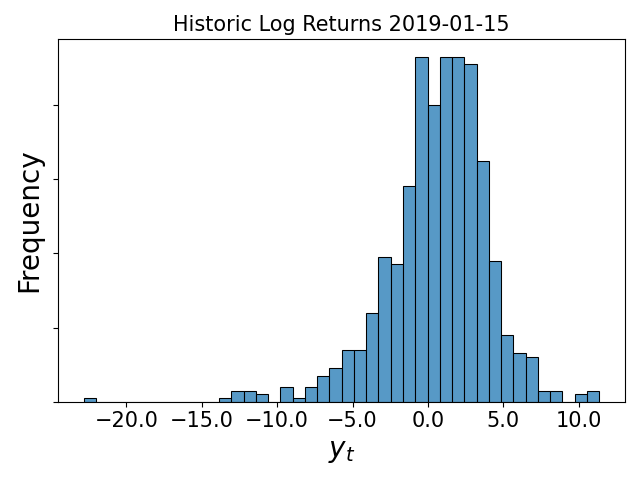
\includegraphics[width=8.5cm]{Graphs/RR_20190115.png}
	\end{minipage}
	\begin{minipage}{0.5\linewidth}
	    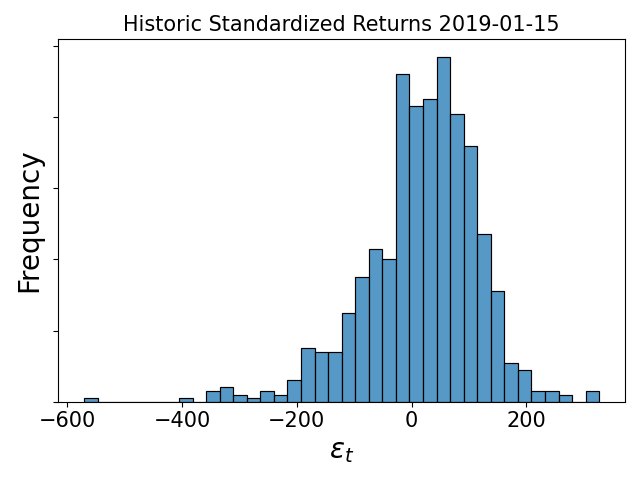
\includegraphics[width=8.5cm]{Graphs/SR_20190115.png}
	\end{minipage}
\label{fig:LogStandRet}
\end{figure}

In order to remove unrealistic data, observations that meet any of these 3 criteria are removed from the CBOE options dataset: (1) zero volume traded; (2) bid price lower than $\$0.125$, (3) bid price lower than ask price. These 3 filters correspond to the columns: 'Volume', 'bid\_eod', and 'ask\_eod' respectively. The data is then filtered for expiration dates that land on the 3rd Friday of each month. Then option quote times are filtered for 1 month to maturity, 28/29/30/31 days depending on the month and year. Figure \ref{fig:ContractCount} shows the number of call and put contracts by date from the CBOE data after filtering.

\begin{figure}[H]
\captionsetup{width=12cm, skip=0pt}
    \begin{center}
    	\caption{\\ \textbf{Count of Option Contracts} \rule{12cm}{0.5pt}\\ \footnotesize{\textit{Count of Contracts by date and by option type after CBOE option data was filtered. Time span is from January 2019 to May 2021.}}}
        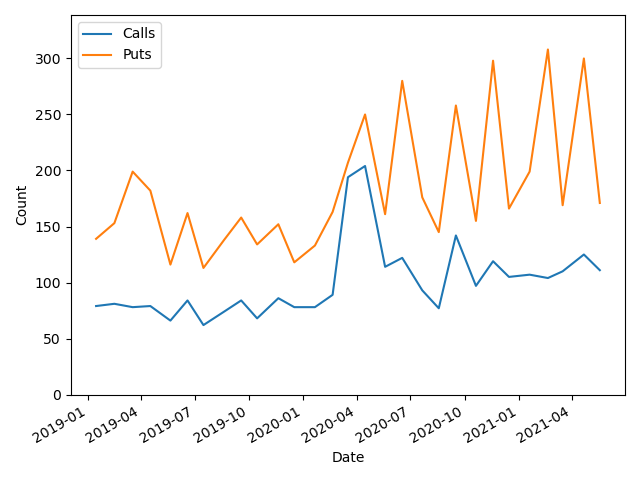
\includegraphics[width=12cm]{Graphs/Contract_Count.png}
        \label{fig:ContractCount}
    \end{center}
\end{figure}

Then I further filter the option contracts used in the portfolio optimization by defining four types of contracts. I define an at-the-money (ATM) call/put and an out-of-the-money (OTM) call/put. ATM calls/puts are found by finding the contract for each date with the lowest bid-ask spread and a moneyness between $-1\% \text{ to } 1\%$. OTM calls/puts are found in the same manner, however with moneyness from $-5\% \text{ to } -2\%$ and $2\% \text{ to } 5\%$ respectively. Figure \ref{fig:Opts_TS} shows a time series of these four contracts option closing prices. While Covid was priced into the OTM/ATM puts in March 2020, it was priced into the ATM call a month earlier in February. This indicates the options market believed the S\&P500 would increase from February to March, while in March, after the underlying price had already dropped significantly, the options market believed that the underlying price would continue to drop.

\begin{figure}[H]
\captionsetup{width=13.2cm, skip=0pt}
    \begin{center}
    	\caption{\\ \textbf{Option Prices Time Series} \rule{13.2cm}{0.5pt}\\ \footnotesize{\textit{Time Series of option closing prices by type of contract. Time span is from January 2019 to May 2021. February 2020 is marked as a dotted line.}}}
        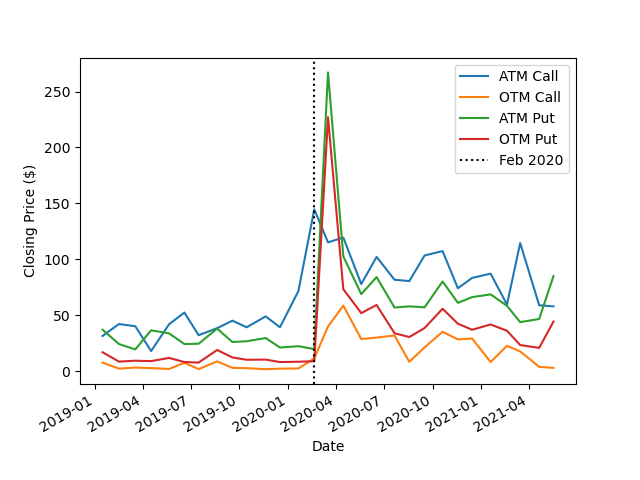
\includegraphics[width=10cm]{Graphs/Opt_Series.png}
        \label{fig:Opts_TS}
    \end{center}
\end{figure}

Table \ref{tab:Table3} shows summary statistics for the realized returns of these four contracts, as well as for an even weighting between the four, the underlying S\&P500, and the risk free asset. Figure \ref{fig:Fig3_kde} shows the histograms of the actual returns of each of the four option contracts, with extreme outliers removed. All four option contracts exhibit a positive skewness, while an ATM call has the lowest skewness and kurtosis of the four contracts. The mean returns of both ATM and OTM puts are larger than ATM calls, due to their large positive tail returns. However their standard deviations lead to lower sharpe ratios than the ATM call. The OTM call has a negative mean return, implying that shorting OTM calls could be a profitable strategy. The positive mean returns of ATM and OTM puts is in contrast to the time period used in \cite{faias2017optimal}, which may be due to the small sample size and the outsized impact of the maximum returns in February 2020.

\begin{table}[H]
\captionsetup{width=12.5cm, skip=5pt}
\begin{center}
	\caption{\\ \textbf{Actual Returns for Options, S\&P500, and Risk Free} \rule{12.5cm}{0.5pt}\\ \footnotesize{\textit{ATM/OTM Call/Put show individual realized option returns for a hold until expiration strategy. $\frac{1}{N}$ shows return for even weighting on each of the four contracts. S\&P500, Risk Free show actual returns for underlying asset and risk free treasury bill respectively. Mean, Std, Min, Max are shown as percentages.}}}
    \scalebox{0.75}{\begin{tabular}{lrrrrrrr}
\hline
                &   Mean &     Std &     Min &     Max &   Skew &   Kurtosis &    SR \\
\hline
 ATM\_Call       &  13.5\% &   98.3\% & -100.0\% &  298.3\% &   0.71 &       0.49 &  0.14 \\
 ATM\_Put        &  19.3\% &  561.8\% & -100.0\% & 2923.5\% &   5.01 &      23.42 &  0.03 \\
 OTM\_Call       & -55.2\% &  122.9\% & -100.0\% &  498.1\% &   3.53 &      12.62 & -0.45 \\
 OTM\_Put        &  89.1\% & 1018.2\% & -100.0\% & 5383.4\% &   5.10 &      24.04 &  0.09 \\
 1/N rule       & -19.6\% &  107.8\% & -100.0\% &  480.8\% &   3.58 &      14.29 & -0.18 \\
 S\&P 500        &   1.8\% &    4.7\% &  -19.1\% &    6.3\% &  -3.14 &      11.59 &  0.38 \\
 1-month T-bill & -14.2\% &   31.6\% & -100.0\% &   44.4\% &  -1.34 &       1.66 & -0.45 \\
\hline
\end{tabular}}
    \label{tab:Table3}
\end{center}
\end{table}

\begin{figure}[H]
\captionsetup{width=13cm, skip=0pt}
    \begin{center}
    	\caption{\\ \textbf{Actual Returns by Option Type} \rule{13cm}{0.5pt}\\ \footnotesize{\textit{Histograms of actual returns by option type for a hold until expiration strategy are presented. Returns are percentages, time spans is from January 2019 to May 2021. Returns larger than 1000\% are removed for clarity.}}}
        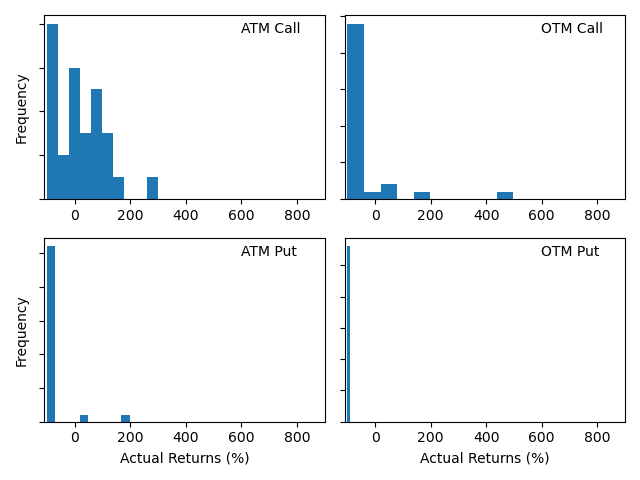
\includegraphics[width=13cm]{Graphs/Fig3_kde.png}
        \label{fig:Fig3_kde}
    \end{center}
\end{figure}

To model the risk free asset, the 1-month treasury bill time series is used. The daily data is downloaded from the Fred St. Louis Database (Ticker "TB4WK"). This data is then joined to match up with the quote time of the options in the filtered CBOE data. This produces a time series of annualized risk free returns, which I convert to monthly returns and take as given in the optimization. Figure \ref{fig:Tbill_TS} shows the time series of the 1-month treasury bill returns. While Figure \ref{fig:Tbill_TS} does not go all the way back to 1996 as in \cite{faias2017optimal}, the average risk-free return from 2001 through 2013 is 1.57 times higher than the risk-free return in the red area, from 2019 through May 2021. As discussed in further detail in section \ref{sec:Results}, this discrepancy may impact a strategy that tends to choose longer positions on the risk free asset.

\begin{figure}[H]
\captionsetup{width=13.2cm, skip=0pt}
    \begin{center}
    	\caption{\\ \textbf{Risk Free Asset Returns} \rule{13.2cm}{0.5pt}\\ \footnotesize{\textit{Time Series of 1-Month Treasury Bill Returns from St. Louis FRED. Time span is from August 2001 to August 2021. Time span of available option data is shown in red.}}}
        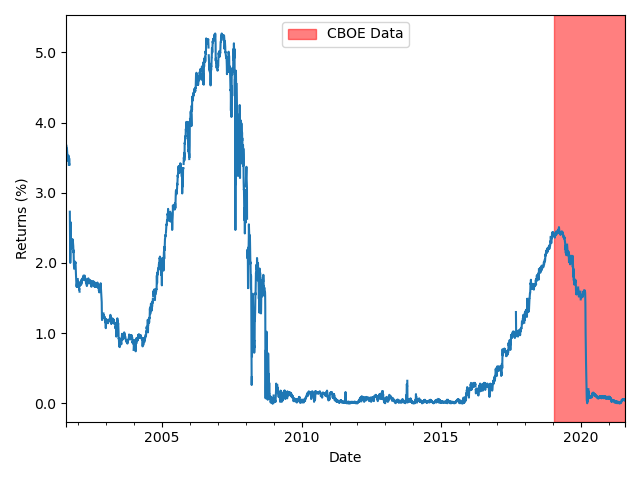
\includegraphics[width=10cm]{Graphs/Tbill_TS.png}
        \label{fig:Tbill_TS}
    \end{center}
\end{figure}

% \clearpage

\section{Estimation}\label{sec:Estimation}

The rolling window GARCH(1, 1) model described in section \ref{sec:GARCH} is estimated using maximum likelihood at a monthly frequency, spanning from December, 2018 to May, 2021. At each time period $t$, the data used to estimate the GARCH model spans from January, 1950 to $t$, inclusive. The estimation results for December, 2018 are shown in Table \ref{tab:ARCH_Mod}. All three coefficients are significantly different from zero, although $\omega$ is 0 out to three decimal points. Additionally, the marginal effect of the squared lag log return ($\alpha$) is lower than the marginal effect of the squared lag conditional volatility ($\beta$).

\begin{table}[H]
	\captionsetup{width=10.5cm, skip=5pt}
	\caption{\\ \textbf{GARCH(1, 1) Log Returns Model} \rule{10.5cm}{0.5pt}\\ \footnotesize{\textit{GARCH(1, 1) model estimation summary is shown. The model is estimated on log returns from January 1950 through December 2018.}}}
    \begin{center}
\begin{tabular}{lcccc}
    & \textbf{coef} & \textbf{std err} & \textbf{t} & \textbf{P$>|$t$|$} \\
\midrule
$\mathbf{\omega}$ & 0.000 & 0.000 & 3.508 & 0.000 \\
$\mathbf{\alpha}$ & 0.125 & 0.038 & 3.309 & 0.001 \\
$\mathbf{\beta}$ & 0.783 & 0.037 & 21.404 & 0.000 \\
\bottomrule
\end{tabular}
\end{center}
    \label{tab:ARCH_Mod}
\end{table}

Figure \ref{fig:GARCH_TS} shows a time series plot of the log returns and the conditional volatility using the rolling GARCH procedure described in Section \ref{sec:GARCH}. The spikes in conditional volatility for the great recession and the Covid pandemic are visible in Figure \ref{fig:GARCH_TS} as well.

\begin{figure}[H]
\captionsetup{width=12cm, skip=0pt}
    \begin{center}
    	\caption{\\ \textbf{GARCH Time Series Plot} \rule{12cm}{0.5pt}\\ \footnotesize{\textit{S\&P500 log returns and GARCH(1, 1) conditional volatility are shown. Period spans from January 1950 to May 2021. After January 2019, conditional volatility values shown are forecasts.}}}
        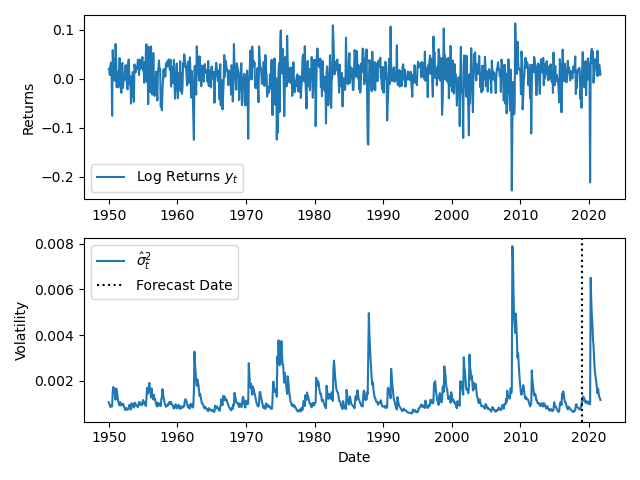
\includegraphics[width=10cm]{Graphs/GARCH_TS_plot.png}
        \label{fig:GARCH_TS}
    \end{center}
\end{figure}

Figure \ref{fig:GARCH_Param} shows a time series of the three GARCH(1, 1) parameters esimated through the rolling scheme. There is some variation in the $\hat{\alpha}$ and $\hat{\beta}$ parameter values across the time period, concentrated in the first 12-18 months, while the $\hat{\omega}$ parameter shows little variation. $\hat{\alpha}$ jumped 25\% from March to April 2020, while $\hat{\beta}$ showed a negligible decline. This can be interpreted that after the Covid shock, the impact of the previous log return value on conditional volatility, through $\hat{\alpha}$, became more important.

\begin{figure}[H]
\captionsetup{width=12cm, skip=0pt}
    \begin{center}
    	\caption{\\ \textbf{GARCH Parameters Time Series} \rule{12cm}{0.5pt}\\ \footnotesize{\textit{GARCH(1, 1) time series of rolling $\hat{\omega}$, $\hat{\alpha}$, and $\hat{\beta}$ parameters. Period spans from December 2018 to August 2021.}}}
        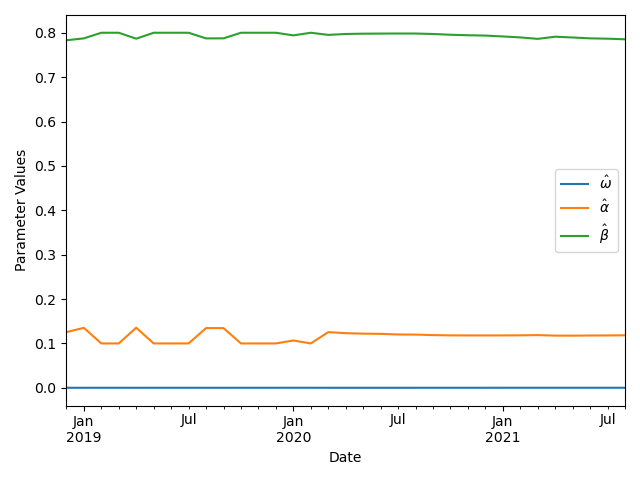
\includegraphics[width=10cm]{Graphs/GARCH_Param_Plot.png}
        \label{fig:GARCH_Param}
    \end{center}
\end{figure}

% \clearpage

\section{Results}\label{sec:Results}
One additional variation of the portfolio optimization technique laid out in section \ref{sec:Model} is now presented. This model introduces a cutoff on the elements of the optimized portfolio weight vector $\mathbf{W}_{t}^{*}$, such that the simulated returns are set to $0$ for contracts whose optimized weights are greater than $10\%$ in absolute value, then the optimization is run again. While setting $\gamma = 10$ does induce some weight shrinkage, this variation models a scenario where a trader enforces a cutoff for their single contract exposure.
\subsection{Portfolio Optimization: Initial Model}\label{sec:PortOpt}
Figure \ref{fig:Fig4_OOPSRet} shows a histogram of the monthly Ex-post returns. We can see that there is a left skewness in the distribution, thus suggesting non-normality of the monthly option returns. Additionally, both the highest and lowest monthly returns are centered around the beginning of the Covid pandemic. The lowest monthly return of -24.2\%, as shown in Table \ref{tab:Table4} and in full detail in Table \ref{tab:Output4} of Appendix \ref{app:Detail}, occurs on the March 2020 expiration, and the highest monthly return of 11.5\% occurs the next month in April 2020. The lowest return is larger in absolute value than the highest.

\begin{figure}[H]
\captionsetup{width=10cm, skip=0pt}
    \begin{center}
   		\caption{\\ \textbf{Portfolio Optimization Returns} \rule{10cm}{0.5pt}\\ \footnotesize{\textit{Histogram of portfolio optimization returns is shown. The time period is January 2019 to May 2021.}}}
        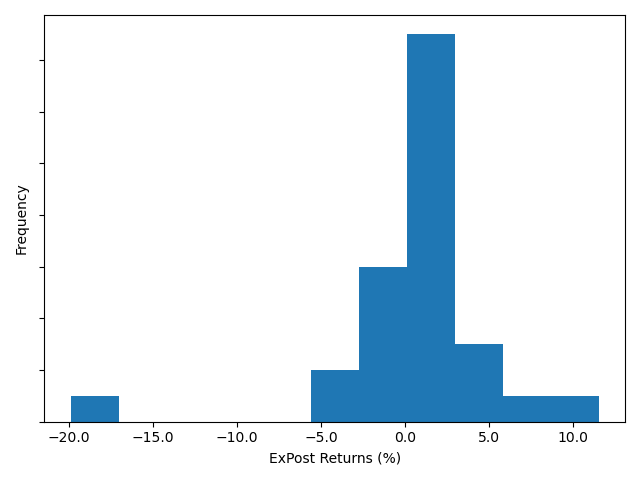
\includegraphics[width=10cm]{Graphs/Fig4_OOPSRet.png}
        \label{fig:Fig4_OOPSRet}
    \end{center}
\end{figure}

Table \ref{tab:Table4} compares the summary of the monthly returns of the option portfolio optimization with the returns of the S\&P500. The Ex-post returns have a mean of -0.2\% and a standard deviation of 5\%, resulting in a lower monthly sharpe ratio than the S\&P500, -0.03 vs. 0.33 in the time period of the data. Additionally, the Ex-post returns have a lower absolute skew and kurtosis, implying that they are closer to normality than the S\&P500 returns.

\begin{table}[H]
\captionsetup{width=13cm, skip=5pt}
\begin{center}
	\caption{\\ \textbf{Portfolio Optimization vs. S\&P500 Returns} \rule{13cm}{0.5pt}\\ \footnotesize{\textit{Summary statistics for the optimized portfolio and S\&P500 returns are shown. The time period is January 2019 to May 2021. Mean, std, min, and max are percentages. The Sharpe Ratio (SR) is monthly.}}}
    \scalebox{0.9}{\begin{tabular}{lrrrrrrr}
\hline
         &   Mean &   Std &   Min &   Max &   Skew &   Kurtosis &   SR \\
\hline
 S\&P 500 &    1.8 &   4.7 & -19.1 &   6.3 &  -3.14 &      11.59 & 0.38 \\
 ExPost  &    0.7 &   5.0 & -19.9 &  11.5 &  -2.22 &       9.15 & 0.15 \\
\hline
\end{tabular}}
    \label{tab:Table4}
\end{center}
\end{table}

Table \ref{tab:Table5} shows the summary statistics of the weights for each type of option contract in the monthly optimization. Contrary to what would be expected from the actual returns by contract in Table \ref{tab:Table3} of Section \ref{sec:Data}, the model is long OTM calls on average, while short on average for ATM calls and OTM puts. Additionally, the range of the weights chosen for the OTM call position, between the minimum and maximum, is much smaller than the other three contracts. Figure \ref{fig:Weights} shows a time series representation of the weights per contract, as well as the risk-free asset weights. This is also shown in detail in Table \ref{tab:Output4} of Appendix \ref{app:Detail}. The risk-free asset weights range from 97\% to 123\% on the March 2020 expiration, where the model exploited the price spike in the ATM call with an extreme short position (-23\%). On average, the portfolio optimization model is a net seller of options, and is in a net short position 83\% of the months. The model overwhelmingly shorts OTM puts, 93\% of the months, with an average short position of -1\%. Lastly, OTM calls generally have a higher weight relative to OTM puts, while this is reversed for ATM calls/puts.

\begin{table}[H]
\captionsetup{width=13cm, skip=5pt}
\begin{center}
	\caption{\\ \textbf{Portfolio Optimization Weights} \rule{13cm}{0.5pt}\\ \footnotesize{\textit{Mean, min, and max are presented for the optimized portfolio weights. The time period is January 2019 to May 2021. All values are percentages.}}}
    \scalebox{0.9}{\begin{tabular}{lrrrr}
\hline
         &   ATM Call &   ATM Put &   OTM Call &   OTM Put \\
\hline
 Mean    &       -2.4 &      -0.0 &        0.5 &      -1.1 \\
 Minimum &      -25.4 &      -3.0 &       -1.9 &      -9.5 \\
 Maximum &        1.7 &       2.9 &        2.1 &       0.3 \\
\hline
\end{tabular}}
    \label{tab:Table5}
\end{center}
\end{table}

\begin{figure}[H]
\captionsetup{width=11cm, skip=0pt}
    \begin{center}
   		\caption{\\ \textbf{Portfolio Optimization Weights by Contract} \rule{11cm}{0.5pt}\\ \footnotesize{\textit{Optimized weights from portfolio optimization are shown by option type, as well as for the call-put difference and risk-free assset. The time period is January 2019 to May 2021.}}}
        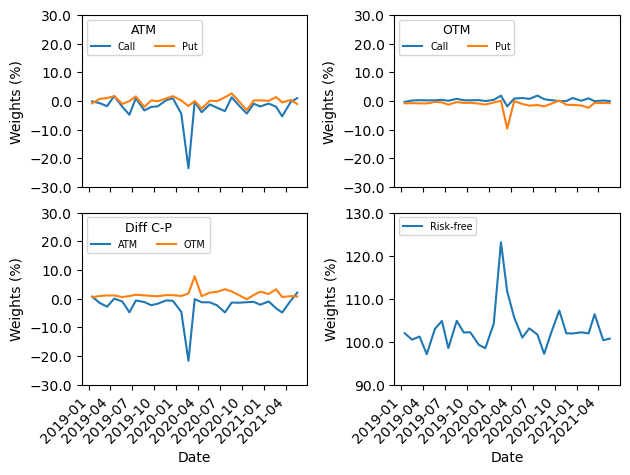
\includegraphics[width=11cm]{Graphs/WeightsPlot.png}
        \label{fig:Weights}
    \end{center}
\end{figure}

Figure \ref{fig:Cum} shows the cumulative returns from January 2019 to May 2021 for the portfolio optimization model, the S\&P500, and the risk-free asset. The initial wealth and February 2020 are marked with dotted lines. Prior to Covid, the cumulative returns of the risk-free asset and the ExPost returns track relatively closely, however, each respond to the Covid shock differently. The risk-free asset levels out, in accordance with Figure \ref{fig:Tbill_TS}, while the Ex-post returns and the S\&P500 both experience steep losses, with the S\&P500 experiencing a 21\% loss. However, the S\&P500 bounces back more quickly, and has the highest ending cumulative return of the three, with the Ex-post returns experiencing a small rebound and then a leveling out.

\begin{figure}[H]
\captionsetup{width=11cm, skip=0pt}
    \begin{center}
   		\caption{\\ \textbf{Cumulative Returns} \rule{11cm}{0.5pt}\\ \footnotesize{\textit{Cumulative returns for portfolio optimization, S\&P500, and risk-free asset are shown. The time period is January 2019 to May 2021, and starting wealth is set to \$100.}}}
        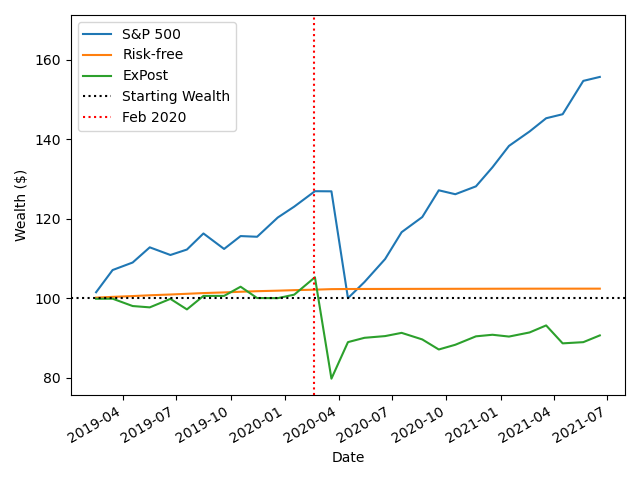
\includegraphics[width=11cm]{Graphs/Cum_Returns.png}
        \label{fig:Cum}
    \end{center}
\end{figure}

% \clearpage

\subsection{Portfolio Optimization: Cutoff Adjusted}\label{sec:PortOpt_Cut}
Figure \ref{fig:Fig4_OOPSRet_Cutoff} displays a histogram of the cutoff adjusted Ex-post returns, and Table \ref{tab:Table4_Cutoff} displays a table comparing these returns to the S\&P500 returns. Contrary to what might be expected, comparing Table \ref{tab:Table4_Cutoff} and Table \ref{tab:Table4}, the largest loss for the cutoff adjusted model is larger in absolute value than the basic model (-28\% vs -24\%). This can be explained by the removal of the large short position in the ATM call from the basic model. While shorting the high price of the ATM call in February 2020 wasn't enough to offset the loss from shorting the ATM put that month, it did partially mitigate it. Additionally, the skew and kurtosis of the cutoff adjusted model are higher as well, meaning it is further from normality than the basic variation.
\begin{figure}[H]
\captionsetup{width=10cm, skip=0pt}
    \begin{center}
   		\caption{\\ \textbf{Portfolio Optimization Returns: Cutoff Adjusted} \rule{10cm}{0.5pt}\\ \footnotesize{\textit{Histogram of portfolio optimization returns is shown. The time period is January 2019 to May 2021. Simulated returns for contracts with weights greater than 10\% in absolute value are forced to zero, and the optimization is rerun.}}}
        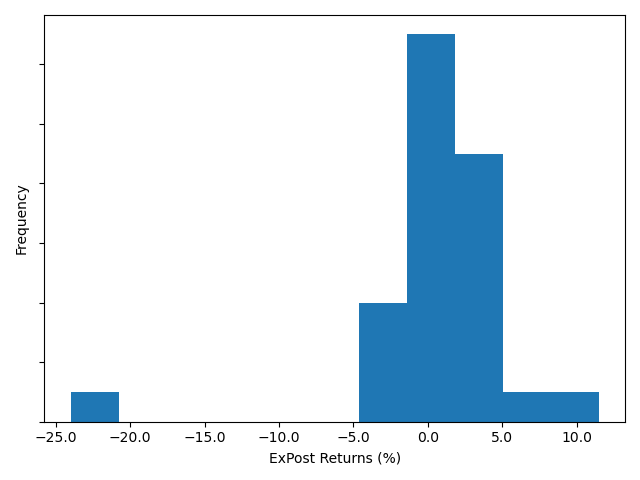
\includegraphics[width=10cm]{Graphs/Fig4_OOPSRet_Cutoff.png}
        \label{fig:Fig4_OOPSRet_Cutoff}
    \end{center}
\end{figure}

\begin{table}[H]
\captionsetup{width=13cm, skip=5pt}
\begin{center}
	\caption{\\ \textbf{Portfolio Optimization vs. S\&P500 Returns: Cutoff Adjusted} \rule{13cm}{0.5pt}\\ \footnotesize{\textit{Summary statistics for the optimized portfolio and S\&P500 returns are shown. The time period is January 2019 to May 2021. Mean, std, min, and max are percentages. The Sharpe Ratio (SR) is monthly. Simulated returns for contracts with weights greater than 10\% in absolute value are forced to zero, and the optimization is rerun.}}}
    \scalebox{0.9}{\begin{tabular}{lrrrrrrr}
\hline
         &   Mean &   Std &   Min &   Max &   Skew &   Kurtosis &    SR \\
\hline
 S\&P 500 &    1.7 &   5.1 & -21.2 &   6.1 &  -3.41 &      13.10 &  0.33 \\
 ExPost  &   -0.3 &   6.1 & -28.5 &  11.5 &  -3.24 &      13.98 & -0.05 \\
\hline
\end{tabular}}
    \label{tab:Table4_Cutoff}
\end{center}
\end{table}

Comparing the optimized weights of the cutoff adjusted model in Table \ref{tab:Table5_Cutoff} with those of the basic model in Table \ref{tab:Table5}, the means are actually fairly similar. Looking at the weights in more detail in Figure \ref{fig:Weights_Cutoff}, we can see the effect of the cutoff adjustment on the risk-free asset weights, which are lower when compared to the basic model in Figure \ref{fig:Weights}. This is especially true in the March 2020 expiration, where the basic model had a more extreme spike (123\% vs. 112\%) in the optimized weight of the risk-free asset. This is due to the discrepancy in the weights of the ATM call on the March 2020 expiration, which was heavily shorted in the basic model (-23.4\% vs. 0\%). Finally, since the loss was actually larger in March 2020 in the cutoff adjusted model (-29\% vs. -24\%), removing the heavily shorted ATM call was not advantageous in this situation. However, favoring the basic model over the cutoff variation due to this result may be a case of overfitting, as reducing an extreme weight may prove profitable in other settings.

\begin{table}[H]
\captionsetup{width=13cm, skip=5pt}
\begin{center}
	\caption{\\ \textbf{Portfolio Optimization Weights: Cutoff Adjusted} \rule{13cm}{0.5pt}\\ \footnotesize{\textit{Mean, min, and max are presented for the optimized portfolio weights. The time period is January 2019 to May 2021. All values are percentages. Simulated returns for contracts with weights greater than 10\% in absolute value are forced to zero, and the optimization is rerun.}}}
    \scalebox{0.9}{\begin{tabular}{lrrrr}
\hline
         &   ATM Call &   ATM Put &   OTM Call &   OTM Put \\
\hline
 Mean    &       -1.5 &       0.2 &        0.3 &      -1.2 \\
 Minimum &       -5.3 &      -3.1 &       -1.8 &      -9.6 \\
 Maximum &        1.8 &       2.7 &        1.9 &       0.2 \\
\hline
\end{tabular}}
    \label{tab:Table5_Cutoff}
\end{center}
\end{table}

\begin{figure}[H]
\captionsetup{width=11cm, skip=0pt}
    \begin{center}
   		\caption{\\ \textbf{Portfolio Optimization Weights by Contract: Cutoff Adjusted} \rule{11cm}{0.5pt}\\ \footnotesize{\textit{Optimized weights from portfolio optimization are shown by option type, as well as for the call-put difference and risk-free assset. The time period is January 2019 to May 2021. Simulated returns for contracts with weights greater than 10\% in absolute value are forced to zero, and the optimization is rerun.}}}
        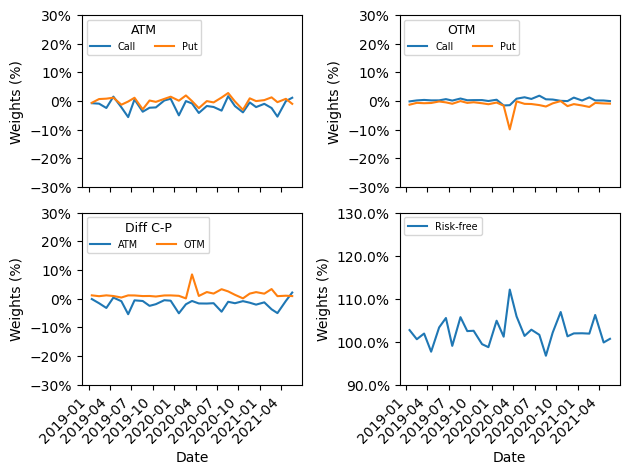
\includegraphics[width=11cm]{Graphs/WeightsPlot_Cutoff.png}
        \label{fig:Weights_Cutoff}
    \end{center}
\end{figure}

Figure \ref{fig:Cum_Cutoff} displays the cumulative returns for a starting wealth of 100\$ for the cutoff adjusted model. The decreased performance of the cutoff adjusted model is visible, where the more extreme loss in March 2020 is visible, and the ending wealth is lower compared to the basic model (\$85.49 vs. \$90.70).

\begin{figure}[H]
\captionsetup{width=11cm, skip=0pt}
    \begin{center}
   		\caption{\\ \textbf{Cumulative Returns: Cutoff Adjusted} \rule{11cm}{0.5pt}\\ \footnotesize{\textit{Cumulative returns for portfolio optimization, S\&P500, and risk-free asset are shown. The time period is January 2019 to May 2021, and starting wealth is set to \$100. Simulated returns for contracts with weights greater than 10\% in absolute value are forced to zero, and the optimization is rerun.}}}
        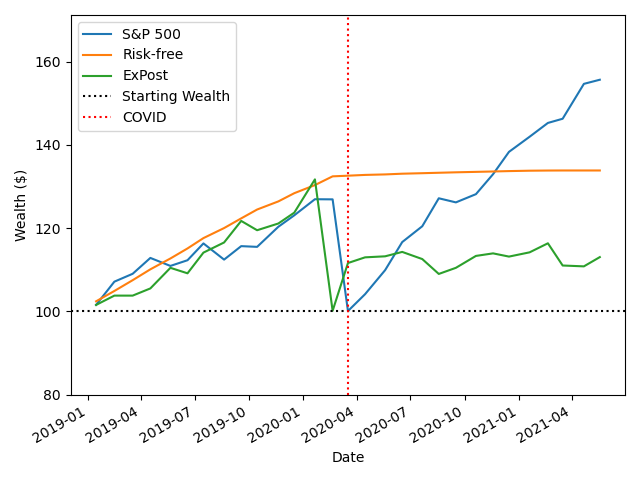
\includegraphics[width=10cm]{Graphs/Cum_Returns_Cutoff.png}
        \label{fig:Cum_Cutoff}
    \end{center}
\end{figure}

\clearpage

\section{Conclusion}\label{sec:Conclusion}

The results of the portfolio optimization model presented in this paper show Ex-post returns which are on average lower compared to both the S\&P500 itself and the risk-free asset. They also show a higher standard deviation and a lower sharpe ratio, in both the basic model and the cutoff adjusted one. However, these returns show a lower skew and kurtosis, implying they are closer to normality than the S\&P500 returns. In both variations, the model chose to hold a net short position which allowed for a greater than 100\% investment in the risk-free asset in 83\% of months. Negative cumulative returns would generally imply a poor choice of model, but there are a couple potential explanations. If February and March of 2020 are excluded, the sharpe ratio of the Ex-post returns is 0.14 in both model variations. This finding provides further evidence that drawing a definite conclusion on the cutoff variation vs. the basic model may constitute overfitting. Additionally, while still lower than the S\&P500, it could mean that a larger sample would smooth out the Covid volatility. Finally, a deeper analysis of the performance of GARCH and other returns forecasting models is beyond the scope of this paper, and would require a longer series of option data to ensure the results are robust.

This paper leaves several extensions open for future research and implementation to transition the option portfolio optimization model to real world trading. Since option contracts can only be traded in integer quantities as opposed to stocks, making the optimization non-convex by imposing an integer constraint would mean the results could be directly traded on. While increasing the computational complexity, these results could be more effectively tested against named option strategies such as the straddles, spreads, and condors described in \cite{chaput2003option}, among others. Additionally, using a dynamic rebalancing strategy rather than held to expiration could prove to be more profitable. This formulation does present some additional challenges, however, if a closed form option pricing is not used to derive an analytical expression for the change in portfolio value. In the case of the GARCH model used in this paper, for example, the future value of the portfolio of options would need to be simulated and appropriately discounted. The dynamically rebalanced portfolio does have some advantages over the static hold until expiration strategy, as noted by \cite{zhao2018markowitz}. Additionally, dynamic rebalancing could occur on any time scale, independent of the expiration date, such as daily or hourly, enabling more trading opportunities. Another extension would be to incorporate further out of the money options, which would increase the choice set in the model, while opening up the issue of low liquidity contracts. To address this, further research could explore creating an effective metric to filter out low liquidity contracts. Lastly, as the skew and kurtosis values of the standardized returns showed only a modest reduction over the log returns in Table \ref{tab:Table1}, the assumption of normality of the standardized returns in the GARCH model in Section \ref{sec:GARCH} may not be valid. Other models to simulate the returns of the underlying asset could also be substituted and tested for their predictive accuracy, including variations on the GARCH, time series methods, or neural networks, among others. 

\clearpage

\nocite{*}
\bibliography{References}

\clearpage

\begin{appendix}
\section{Options Overview}\label{app:Options}

Options are a type of financial derivative. The two types of basic options, calls and puts, give the purchaser the right but not the obligation to buy or sell, respectively, the underlying security at a future date and specified price. With a European option, the holder of the option can exercise their position at the expiration date if they so choose.\footnote{An American option, not considered in this paper, gives the option holder the right to exercise at any time. This early exercise ability makes the American option price higher than is European counter part. Closed form option pricing models such as Black Scholes assume European options.} The seller, or writer, of the options must fulfill their end of the contract if the option is exercised. As with stocks, buying an option is known as taking a long position, and selling a short position.

The buyer of an option increases their choice set, thereby mitigating risk on the downside for a call, and the upside for a put. The seller takes on the risk that the buyer will exercise their option. Therefore, a buyer should pay the seller a cost for this shifting of risk. The price payed for this exchange of risk is the option price.

The price at which the option holder has the right to buy or sell the underlying security is called the strike price, commonly denoted $K$. The time in days until maturity of the option, at its expiration date, is denoted $T$. The price of the option is denoted $C$ and $P$ for calls and puts respectively, as in \cite{faias2017optimal}. The price of the underlying asset at expiration is denoted $S_{T}$. Option moneyness is defined as $\frac{S_{t}}{K} - 1$.

Figures \ref{fig:LC} and \ref{fig:LP} show the profit functions of a long call and a long put respectively. The profit functions of the short side of each of these is obtained by multiplying by $-1$.

\begin{figure}[!htb]
    \begin{minipage}{0.4\linewidth}
        The Profit is

        \[max(X_{t} - K_{i}, 0) - C_{i} = (X_{t} - K_{i})^{+} - C_{i}\]

    \end{minipage}
    \begin{minipage}{0.65\linewidth}
        \centering
        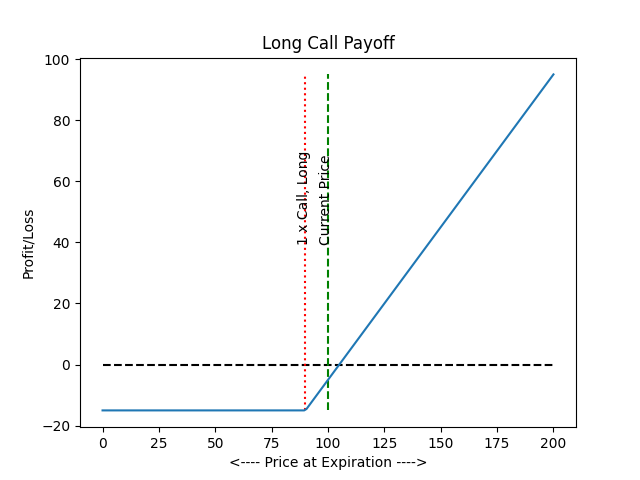
\includegraphics[width=10cm]{Graphs/LongCallEx.png}
        \caption{}
        \label{fig:LC}
    \end{minipage}
\end{figure}

\begin{figure}[!h]
    \begin{minipage}{0.4\linewidth}

        The Profit is

        \[max(K_{i} - X_{t}, 0) - P_{i} = (K_{i} - X_{t})^{+} - P_{i}\]

    \end{minipage}
    \begin{minipage}{0.65\linewidth}
        \centering
        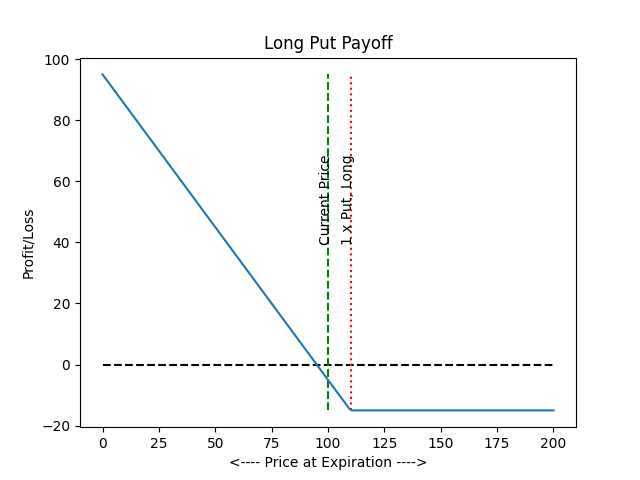
\includegraphics[width=10cm]{Graphs/LongPutEx.png}
        \caption{}
        \label{fig:LP}
    \end{minipage}
\end{figure}
\clearpage
\section{Detailed ExPost Returns}\label{app:Detail}
\begin{table}[H]
\captionsetup{width=13cm, skip=5pt}
\begin{center}
	\caption{\\ \textbf{Detailed Portfolio Optimization Returns} \rule{13cm}{0.5pt}\\ \footnotesize{\textit{ExPost returns, and weights for each of the four contracts and the risk free asset are shown. All values are in percentages.}}}
    \scalebox{0.8}{\begin{tabular}{llrrrrrr}
\hline
 Date       & Expiry     &   ExPost &   ATM\_Call\_Weight &   OTM\_Call\_Weight &   ATM\_Put\_Weight &   OTM\_Put\_Weight &   RfWeight \\
\hline
 2019-01-15 & 2019-02-15 &    -6.3\% &             -4.0\% &              0.6\% &             2.6\% &            -2.6\% &     103.3\% \\
 2019-02-15 & 2019-03-15 &    -3.0\% &             -7.5\% &             -0.7\% &            11.3\% &            -4.6\% &     101.6\% \\
 2019-03-18 & 2019-04-18 &    -5.8\% &             -7.5\% &              1.0\% &             2.9\% &            -1.8\% &     105.5\% \\
 2019-04-17 & 2019-05-17 &    10.5\% &             -5.0\% &              1.3\% &             6.5\% &            -1.9\% &      99.2\% \\
 2019-05-21 & 2019-06-21 &     2.8\% &              1.9\% &              0.3\% &            -1.8\% &             0.0\% &      99.5\% \\
 2019-06-19 & 2019-07-19 &    -5.2\% &             -9.6\% &              1.2\% &             0.9\% &            -0.8\% &     108.3\% \\
 2019-07-16 & 2019-08-16 &    22.9\% &             -8.1\% &              1.1\% &             5.7\% &            -2.4\% &     103.7\% \\
 2019-08-20 & 2019-09-20 &     4.5\% &              3.1\% &              1.4\% &            -1.2\% &            -1.2\% &      97.9\% \\
 2019-09-18 & 2019-10-18 &    11.5\% &            -12.4\% &              1.6\% &             5.5\% &            -3.9\% &     109.3\% \\
 2019-10-15 & 2019-11-15 &    -1.9\% &             -2.6\% &              0.4\% &            -0.3\% &            -0.5\% &     103.0\% \\
 2019-11-20 & 2019-12-20 &   -12.2\% &            -12.0\% &              1.1\% &             6.7\% &            -3.2\% &     107.5\% \\
 2019-12-17 & 2020-01-17 &    -7.7\% &             -5.7\% &              0.5\% &             4.0\% &            -2.3\% &     103.5\% \\
 2020-01-21 & 2020-02-21 &    18.1\% &            -19.2\% &              1.4\% &             3.3\% &            -1.9\% &     116.4\% \\
 2020-02-20 & 2020-03-20 &    -7.7\% &            -43.8\% &              3.9\% &            -5.6\% &             2.1\% &     143.3\% \\
 2020-03-17 & 2020-04-17 &   603.3\% &             -2.0\% &              0.7\% &          -602.9\% &             0.0\% &     704.2\% \\
 2020-04-15 & 2020-05-15 &    -3.4\% &            -10.6\% &              3.5\% &             2.8\% &            -3.6\% &     108.0\% \\
 2020-05-19 & 2020-06-19 &    -5.2\% &             -2.2\% &              0.2\% &            19.5\% &           -16.7\% &      99.1\% \\
 2020-06-17 & 2020-07-17 &    -4.7\% &            -12.9\% &              3.4\% &            13.0\% &           -11.1\% &     107.5\% \\
 2020-07-21 & 2020-08-21 &    -6.6\% &             -8.4\% &              3.2\% &             3.1\% &            -2.2\% &     104.2\% \\
 2020-08-18 & 2020-09-18 &     2.2\% &             -6.4\% &              1.1\% &             7.8\% &            -4.6\% &     102.1\% \\
 2020-09-16 & 2020-10-16 &     0.7\% &             -5.2\% &              2.6\% &             2.7\% &            -2.9\% &     102.8\% \\
 2020-10-20 & 2020-11-20 &    -0.5\% &             -7.6\% &              1.1\% &             3.2\% &            -4.2\% &     107.5\% \\
 2020-11-18 & 2020-12-18 &   -10.5\% &            -13.4\% &              4.8\% &            10.9\% &            -9.2\% &     106.9\% \\
 2020-12-15 & 2021-01-15 &    -3.4\% &             -2.2\% &             -0.7\% &             9.1\% &            -6.4\% &     100.1\% \\
 2021-01-19 & 2021-02-19 &    -2.0\% &             -7.0\% &              0.8\% &             4.5\% &            -4.1\% &     105.8\% \\
 2021-02-19 & 2021-03-19 &     6.6\% &            -11.0\% &              4.3\% &             3.0\% &            -2.9\% &     106.6\% \\
 2021-03-16 & 2021-04-16 &    -5.9\% &             -6.1\% &              0.5\% &             1.8\% &            -1.8\% &     105.6\% \\
 2021-04-21 & 2021-05-21 &     3.6\% &            -11.2\% &              1.8\% &            12.7\% &            -6.9\% &     103.6\% \\
 2021-05-18 & 2021-06-18 &     1.6\% &             -1.7\% &              0.3\% &            -1.1\% &            -0.7\% &     103.2\% \\
\hline
\end{tabular}}
    \label{tab:Output4}
\end{center}
\end{table}

\begin{table}[H]
\captionsetup{width=13cm, skip=5pt}
\begin{center}
	\caption{\\ \textbf{Detailed Portfolio Optimization Returns: Cutoff} \rule{13cm}{0.5pt}\\ \footnotesize{\textit{ExPost returns, and weights for each of the four contracts and the risk free asset are shown for the cutoff variation. All values are in percentages.}}}
    \scalebox{0.8}{\begin{tabular}{llrrrrrr}
\hline
 Date       & Expiry     &   ExPost &   ATM Call &   OTM Call &   ATM Put &   OTM Put &   Risk Free \\
\hline
 2019-01-15 & 2019-02-15 &     -0.1 &       -0.1 &       -0.3 &      -0.8 &      -0.8 &       102.0 \\
 2019-02-15 & 2019-03-15 &      0.0 &       -0.7 &        0.2 &       0.8 &      -0.7 &       100.5 \\
 2019-03-18 & 2019-04-18 &     -1.8 &       -1.8 &        0.3 &       1.0 &      -0.8 &       101.2 \\
 2019-04-17 & 2019-05-17 &     -0.3 &        1.8 &        0.2 &       1.7 &      -0.8 &        97.1 \\
 2019-05-21 & 2019-06-21 &      2.2 &       -2.0 &        0.3 &      -1.0 &      -0.3 &       103.0 \\
 2019-06-19 & 2019-07-19 &     -2.7 &       -4.8 &        0.4 &       0.0 &      -0.5 &       104.8 \\
 2019-07-16 & 2019-08-16 &      3.5 &        1.0 &        0.1 &       1.6 &      -1.3 &        98.5 \\
 2019-08-20 & 2019-09-20 &      0.0 &       -3.2 &        0.8 &      -2.1 &      -0.3 &       104.8 \\
 2019-09-18 & 2019-10-18 &      2.3 &       -2.0 &        0.3 &       0.3 &      -0.7 &       102.1 \\
 2019-10-15 & 2019-11-15 &     -2.8 &       -1.8 &        0.3 &      -0.0 &      -0.6 &       102.2 \\
 2019-11-20 & 2019-12-20 &     -0.0 &        0.3 &        0.3 &       0.9 &      -0.9 &        99.3 \\
 2019-12-17 & 2020-01-17 &      0.9 &        1.0 &        0.0 &       1.7 &      -1.2 &        98.5 \\
 2020-01-21 & 2020-02-21 &      4.3 &       -4.4 &        0.4 &       0.2 &      -0.5 &       104.2 \\
 2020-02-20 & 2020-03-20 &    -28.5 &        0.0 &       -1.6 &       1.8 &      -1.6 &       101.4 \\
 2020-03-17 & 2020-04-17 &     11.5 &       -0.2 &       -1.8 &      -0.0 &      -9.6 &       111.6 \\
 2020-04-15 & 2020-05-15 &      1.2 &       -3.9 &        0.9 &      -2.6 &      -0.0 &       105.7 \\
 2020-05-19 & 2020-06-19 &      0.5 &       -1.2 &        1.1 &       0.1 &      -1.0 &       101.0 \\
 2020-06-17 & 2020-07-17 &      0.9 &       -2.3 &        0.8 &      -0.0 &      -1.6 &       103.1 \\
 2020-07-21 & 2020-08-21 &     -1.8 &       -3.5 &        1.9 &       1.3 &      -1.4 &       101.6 \\
 2020-08-18 & 2020-09-18 &     -2.8 &        1.3 &        0.7 &       2.7 &      -1.8 &        97.2 \\
 2020-09-16 & 2020-10-16 &      1.4 &       -1.4 &        0.3 &      -0.0 &      -0.9 &       102.1 \\
 2020-10-20 & 2020-11-20 &      2.4 &       -4.4 &       -0.0 &      -3.1 &       0.2 &       107.2 \\
 2020-11-18 & 2020-12-18 &      0.4 &       -0.9 &        0.0 &       0.2 &      -1.3 &       102.0 \\
 2020-12-15 & 2021-01-15 &     -0.5 &       -1.9 &        1.1 &       0.3 &      -1.4 &       101.9 \\
 2021-01-19 & 2021-02-19 &      1.1 &       -0.9 &        0.1 &       0.1 &      -1.5 &       102.2 \\
 2021-02-19 & 2021-03-19 &      1.9 &       -2.0 &        1.0 &       1.4 &      -2.3 &       101.9 \\
 2021-03-16 & 2021-04-16 &     -4.8 &       -5.3 &       -0.0 &      -0.5 &      -0.6 &       106.4 \\
 2021-04-21 & 2021-05-21 &      0.3 &       -0.3 &        0.2 &       0.4 &      -0.7 &       100.3 \\
 2021-05-18 & 2021-06-18 &      1.9 &        1.0 &        0.0 &      -1.0 &      -0.7 &       100.7 \\
\hline
\end{tabular}}
    \label{tab:Output4_Cutoff}
\end{center}
\end{table}
\end{appendix}

\end{document}



